\section{Methodik}\label{chap:Methodik}

Aufgrund ihrer Wichtigkeit für diese Arbeit werden zunächst die verwendeten Netztopologien sowie deren Clusterung zur Bestimmung repräsentativer Netze, anhand welcher die Untersuchungen vorgenommen werden, beschrieben und vorgestellt.
Anschließend werden mit Hilfe des Software Tools \glsi{SIMBEV} Fahrtprofile von \glspl{EPKW} erstellt und der Ladebedarf räumlich auf eine georeferenzierte Ladeinfrastruktur verteilt.
Daraufhin werden abhängig von der Ladestrategie Lastzeitreihen erstellt und in die Netzmodelle integriert.
Abschließend werden etwaige Netzprobleme bestimmt und der Abregelungsbedarf ermittelt, welcher nötig ist, um diese aufzulösen.


\subsection{Verwendete Verteilnetztopologien}\label{chap:dingo_theo}

Eine der Grundlagen für die Nutzung des Netzplanungsinstruments \glsipl{EDISGO} sind die zu untersuchenden Netztopologien mitsamt der \gls{MS}- und \gls{NS}-Ebene.
Aufgrund der mangelnden Datenlagen von realen Netztopologien, wird auf synthetisch erzeugte Netztopologien zurückgegriffen, die innerhalb des \glsi{OPENEGO} Projektes \cite{Mueller2019} mit Hilfe des Open Source Tools \glsi{DINGO} erzeugt wurden.
Das Tool ist in der Lage ländliche und suburbane Netzstrukturen für Gesamtdeutschland zu synthetisieren und kann auf \textit{GitHub} \cite{dingo2019} öffentlich eingesehen und frei verwendet werden.
Weiterhin ist auf \textit{Read the Docs} \cite{dingo-docs2019} eine ausführliche Dokumentation hinterlegt.
Urbane Netzgebiete können derzeit nicht durch \glsi{DINGO} abgebildet und deshalb nicht innerhalb dieser Arbeit betrachtet werden.\medskip


\subsubsection{Auswahl repräsentativer Verteilnetztopologien}

Auf der \gls{MS}-Ebene werden \num{3354} Netzgebiete \cite{Schachler} identifiziert.
\autoref{fig:grid_176_map} zeigt den Aufbau eines beispielhaften Mittelspannungsnetzes, welches mit Hilfe von \glsi{DINGO} erzeugt wurde und innerhalb dieser Arbeit untersucht wird.

\begin{figure}[H]
    \centering
    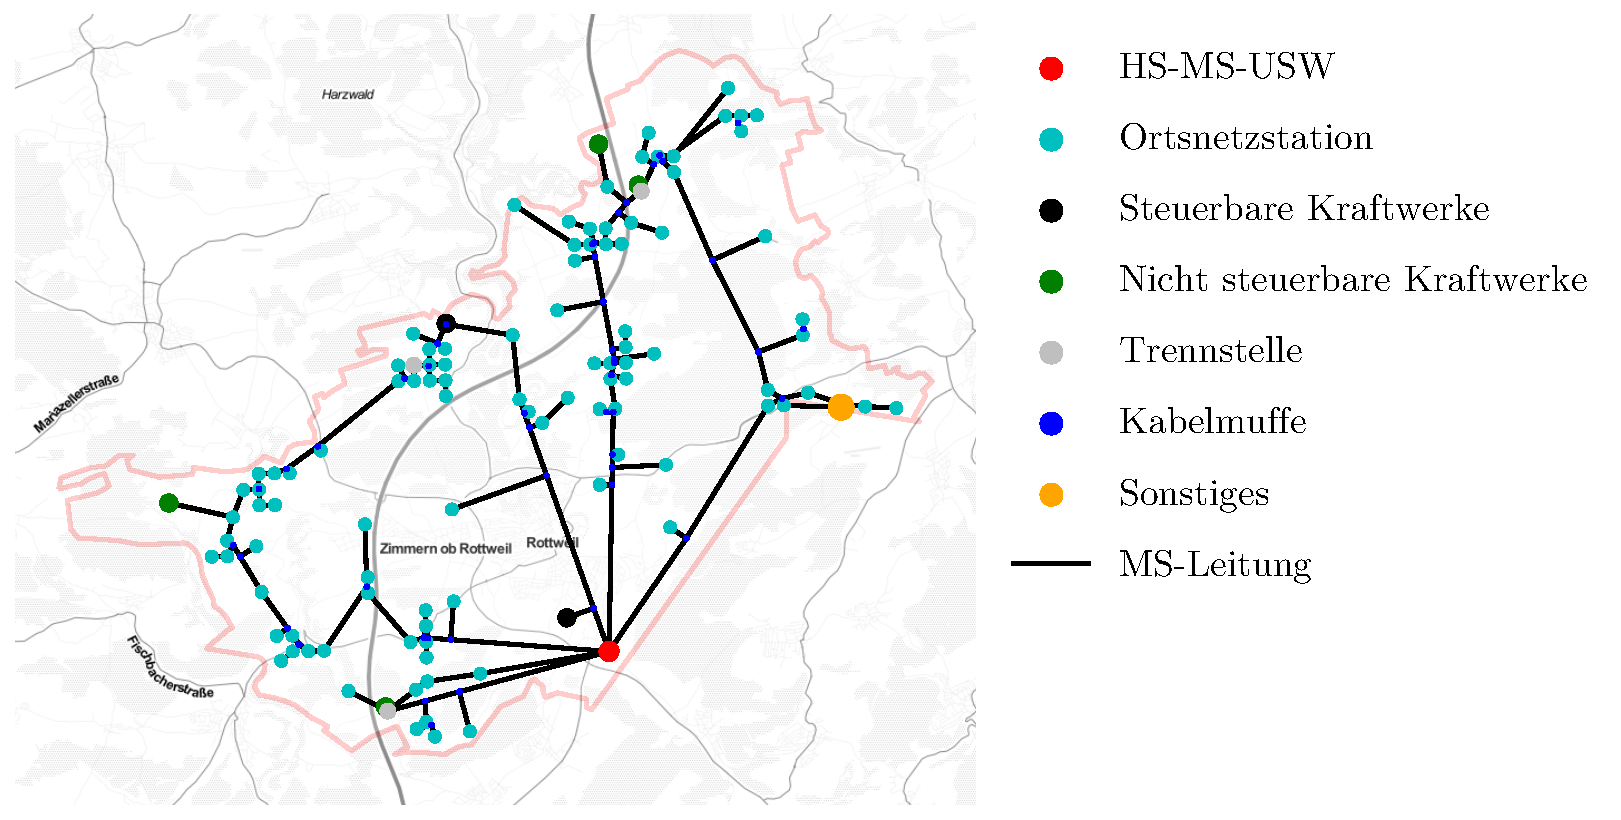
\includegraphics[width=\textwidth]{Bilder/grid_176_map}
    \caption{Beispielhafte Darstellung des MS-Netzes \num{176} mit allen Umspannwerken, Erzeugerkapazitäten und sonstigen Betriebsmitteln}\label{fig:grid_176_map}
\end{figure}

Bei der Synthese der Netztopologien wird auf eine hohe räumliche und zeitliche Auflösung der Netzdatenmodelle geachtet.
Die große Anzahl an Netzgebieten und die hohe Auflösung führen zu inakzeptabel hohen Rechenzeiten.
Um die Komplexität des Modells zu reduzieren, werden in der \textit{E-Mobility Study} \cite{Schachler} mit Hilfe des \mbox{\kmeans} Referenznetzgebiete ausgewählt, die jeweils stellvertretend für eine große Anzahl an Netzgebieten stehen.
Das \mbox{\kmean} wurde im Rahmen des \glsi{OPENEGO} Projektes entwickelt und eine ausführliche Beschreibung der Methodik findet sich im Projektabschlussbericht \cite{Mueller2019}.\medskip

Um mit dieser Arbeit eine Ergänzung zu der \textit{E-Mobility Study} \cite{Schachler} zu liefern, werden die Ergebnisse des Clusterings aus der \textit{E-Mobility Study} übernommen und von den \num{15} identifizierten repräsentativen Netzgebieten eine Teilmenge untersucht.
So werden jeweils zwei Netzgebiete der Kategorien \gls{PV}- und Wind-dominiert sowie ein Netzgebiet der Kategorie Last-dominiert ausgewählt, die stellvertretend für viele Netzgebiete stehen.
Auf diese Weise wird sichergestellt, dass die Effekte der Netzintegration der Elektromobilität für möglichst unterschiedliche Netzklassen aufgezeigt werden können.
Insgesamt werden somit fünf Netzgebiete untersucht, die repräsentativ für \num{1495} der \num{3354} Netzgebiete stehen.
In \autoref{tab:grid_IDs} ist die jeweilige Kategorie und die Anzahl an repräsentierten Netzgebieten der untersuchten Referenznetzgebiete dargestellt.
Der Index der Netz \glspl{ID} steht hierbei für die jeweilige Netzkategorie.

{
\renewcommand{\arraystretch}{1.2}% grßerer Zeilenabstand
\sisetup{range-phrase=~{--}~}% Gedankenstrich statt "bis" bei SIrange
\begin{table}[H]
	\begin{center}
		\caption{Anzahl der repräsentierten Netzgebiete und Kategorie der untersuchten Mittelspannungsnetze}
		\begin{tabu} to \textwidth {X[1] X[1] X[1, r] }
			\hline
			Netz ID    & Kategorie      & Anzahl repräsentierter Netze \\ \hline
			\num{176}  & PV-dominiert   & \num{413}                    \\
			\num{1056} & PV-dominiert   & \num{197}                    \\
			\num{1690} & Wind-dominiert & \num{141}                    \\
			\num{1811} & Wind-dominiert & \num{78}                     \\
			\num{177}  & Last-dominiert & \num{666}                    \\
			\num{2534} & Last-dominiert & \num{347}                    \\ \hline
		\end{tabu}
		\label{tab:grid_IDs}
	\end{center}
	\vspace{-3mm}%Put here to reduce too much white space after your table
\end{table}
}

In \autoref{fig:bar_representatives} sind die wichtigsten Charakteristika der untersuchten Referenznetzgebiete dargestellt.
Hierzu zählen die installierten \gls{PV}-, Wind- und sonstigen Erzeuger-Kapazitäten, sowie die Spitzenlast der \glspl{EPKW} beim Referenz-Laden (s. \autoref{chap:theo_strategies}) im Antriebswende-Szenario (s. \autoref{chap:Szenariorahmen}) und des konventionellen Stromverbrauches inklusive \glspl{WP}.
Weiterhin wird in \autoref{fig:map_representatives} eine Karte der repräsentierten Netzgebiete, eingeteilt in die Kategorien \gls{PV}-, Wind- und Last-dominiert, dargestellt.

\begin{figure}[H]
    \centering
    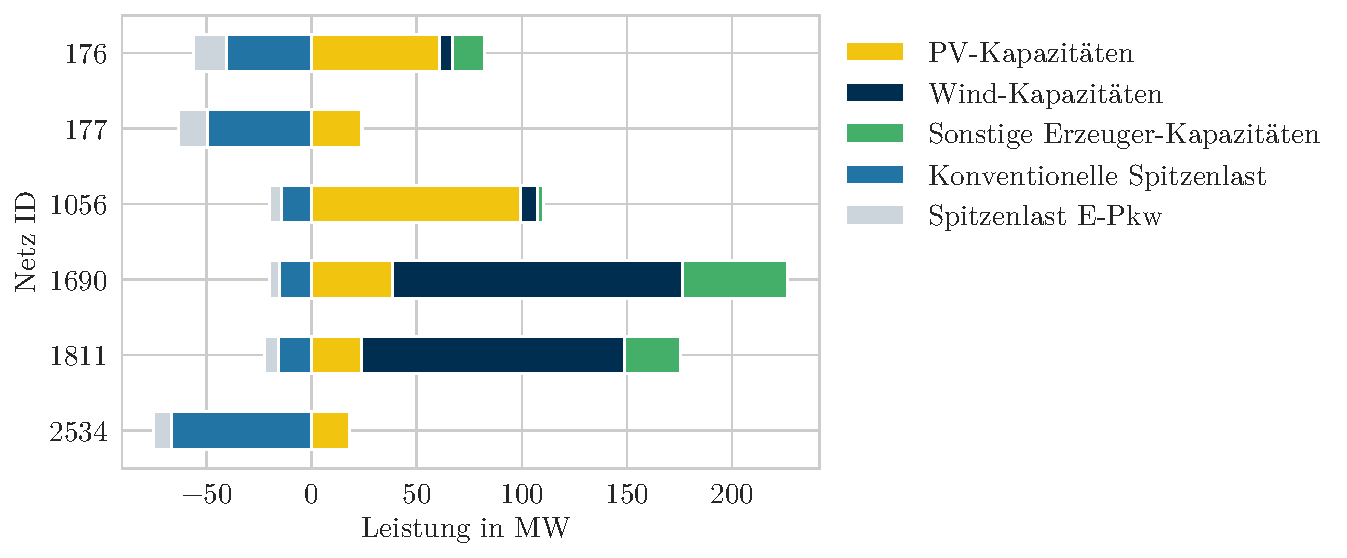
\includegraphics[width=\textwidth]{Bilder/Installed_cap_peak_load_representatives}
    \caption{Kumulierte Wirkleistung von PV-, Wind- und sonstigen Erzeuger-Kapazitäten sowie die kumulierte konventionelle und mobilitätsbedingte Spitzenlast in den Referenznetzgebieten}\label{fig:bar_representatives}
\end{figure}

\begin{figure}[H]
    \centering
    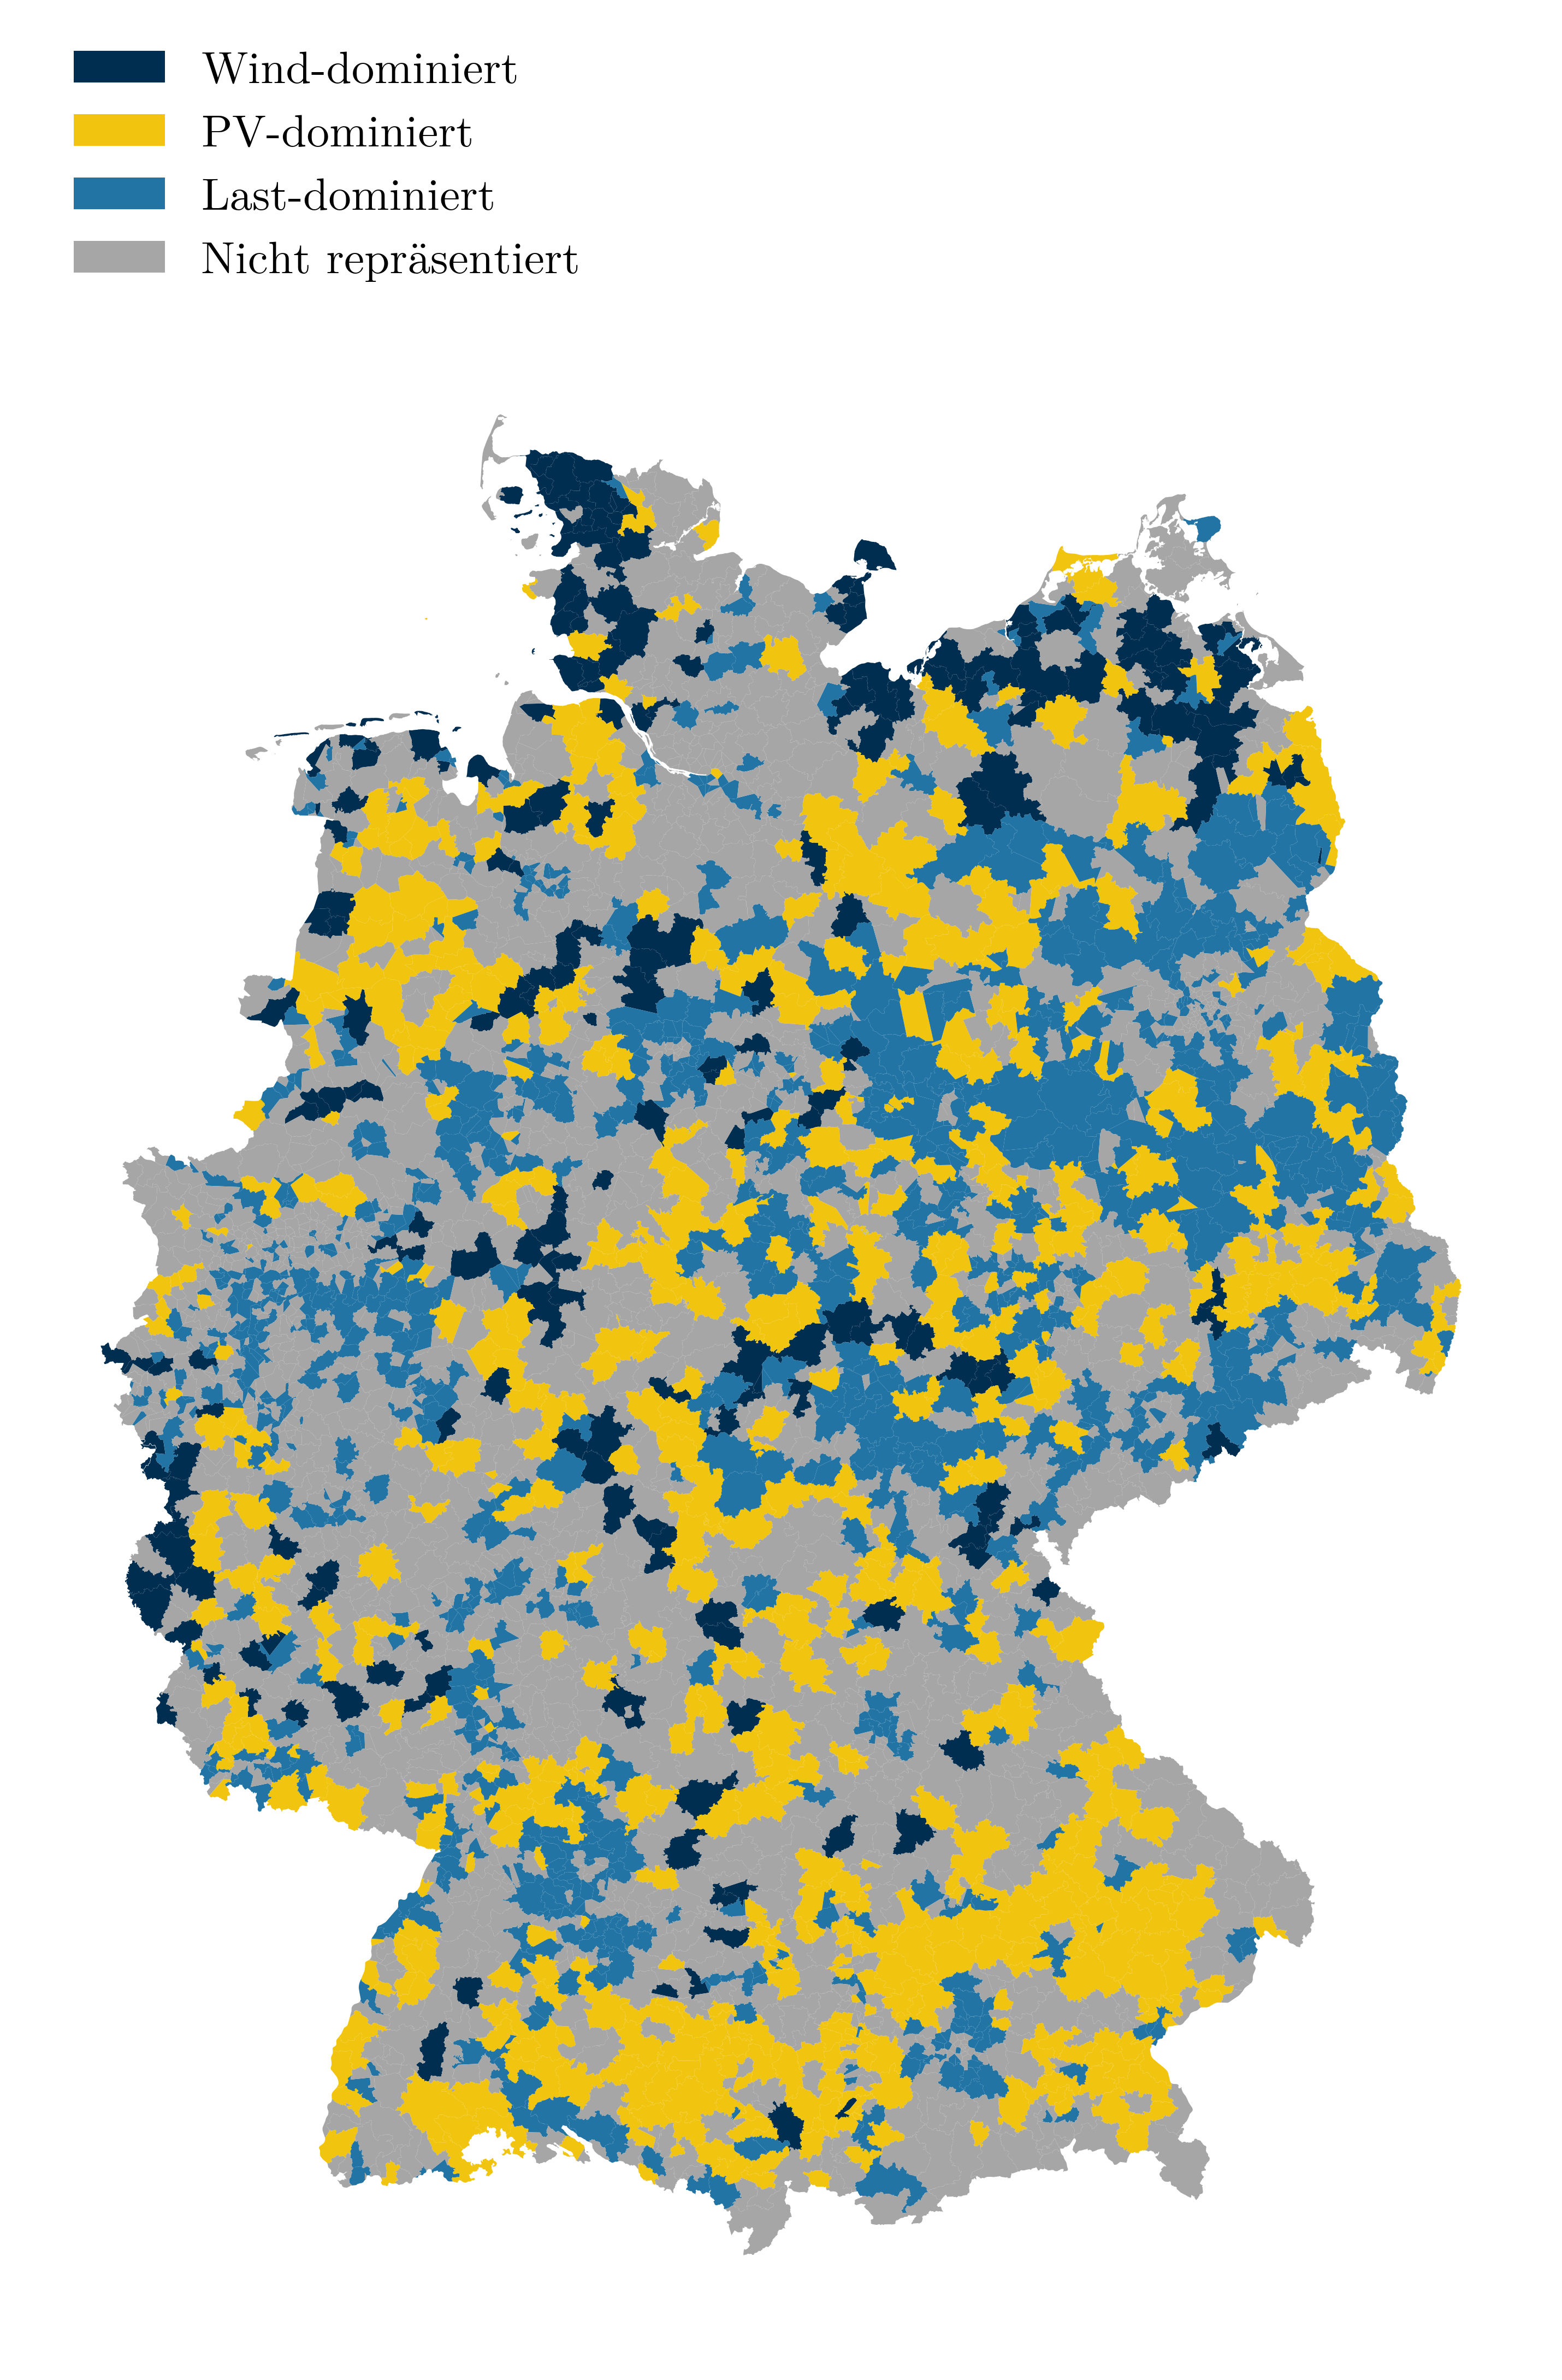
\includegraphics[width=\textwidth]{Bilder/clusters_representatives}
    \caption{Repräsentierte Netzgebiete in Deutschland}\label{fig:map_representatives}
\end{figure}


\subsubsection{Netzausbau}

In der konventionellen Netzplanung werden Betriebsmittel in der Regel überdimensioniert ausgelegt, um die Versorgungsaufgabe für eine möglichst lange Betriebszeit zu garantieren.
Da die Netzgebiete des \glsi{OPENEGO} Projektes so ausgebaut werden, dass die Versorgungsaufgabe des Jahres \num{2015} möglichst genau erfüllt werden kann, werden die Netzgebiete innerhalb dieser Arbeit zusätzlich ausgebaut.
Es wird angenommen, dass die Betriebsmittel mit einem Überdimensionierungsfaktor für die Scheinleistungs- bzw. Stromstärkenbelastbarkeit von mindestens \num{1.3} geplant werden und dementsprechend ausgebaut.
Dies gilt sowohl für die Transformator-Stationen als auch die Kabel innerhalb des Netzgebietes.
Die verwendeten Betriebsmittel können der Dokumentation \glsipl{EDISGO} \cite{edisgoDocs2017a} entnommen werden.
Sollte die maximal auftretende Scheinleistungsbelastung einer Transformator-Station größer sein als der größte verfügbare Transformator, so werden entsprechend benötigte Transformatoren parallel betrieben, um den Anforderungen gerecht zu werden.


\subsection{Erstellung der Fahrtprofile der E-Pkw}\label{chap:simbev_theo}

Mit Hilfe des im Rahmen dieser Arbeit mitentwickelten Software Tools \glsi{SIMBEV} können die Fahrtprofile für eine beliebige Anzahl an \glspl{EPKW} verschiedener Fahrzeugklassen erstellt werden.
Grundlage von \glsi{SIMBEV} bildet die Befragung \glsi{MID} \cite{ISGH2017}.
Nachfolgend wird zunächst die Datengrundlage und anschließend die Methodik zur Erstellung der Fahrtprofile mit Hilfe von \glsi{SIMBEV} beschrieben.


\subsubsection{Mobilität in Deutschland}\label{chap:MID}

Das Ziel der Befragung \glsi{MID} \cite{ISGH2017} ist es, eine Datengrundlage für das alltägliche Mobilitätsverhalten von Personen und Haushalten über ein Jahr zu bilden.
Für diese Arbeit sind vor allem die Erhebungen der sieben Hauptwegezwecke entscheidend.
Diese sind: \textit{Arbeit}, \textit{dienstlich}, \textit{Ausbildung}, \textit{Einkauf}, \textit{Erledigung}, \textit{Freizeit} und \textit{Begleitung}.
In \autoref{tab:wegezweck} wird die prozentuale Aufteilung der Hauptwegezwecke am \gls{PKW}-Verkehrsaufkommen in Wegen beschrieben.

{
\renewcommand{\arraystretch}{1.2}% grßerer Zeilenabstand
\sisetup{range-phrase=~oder~}
\begin{table}[H]
	\begin{center}
		\caption{Anteil der Fahrtzwecke am Pkw-Verkehrsaufkommen (Wege)}
		\begin{tabu} to 0.6\textwidth {X[1] X[1, r]}
			\hline
			Wegezweck  & Verkehrsaufkommen \\ \hline
			Arbeit     & \SI{28}{\percent} \\
			dienstlich & \SI{21}{\percent} \\
			Ausbildung & \SI{1}{\percent}  \\
			Einkauf    & \SI{8}{\percent}  \\
			Erledigung & \SI{13}{\percent} \\
			Freizeit   & \SI{24}{\percent} \\
			Begleitung & \SI{6}{\percent}  \\ \hline
            \multicolumn{2}{l}{Quelle: \cite{Nobis2019}}
		\end{tabu}
		\label{tab:wegezweck}
	\end{center}
	\vspace{-3mm}%Put here to reduce too much white space after your table
\end{table}
}

Der Wegezweck \textit{Begleitung} wird innerhalb von \glsi{SIMBEV} nicht abgebildet, da hierfür keine zusätzliche Fahrt angetreten wird.
Der Rückweg der Wegezwecke wird getrennt als Wegezweck \nH berücksichtigt, da dem Laden zu Hause eine besonders wichtige Rolle beim Laden der \glspl{EPKW} zukommt.
Weiterhin dient \glsi{SIMBEV} nur der Erstellung von Fahrtprofilen für \glspl{PKW}, weshalb ausschließlich die Ergebnisse der Befragung zu Fahrten mit dem Hauptverkehrsmittel \gls{PKW} betrachtet werden.
Die für diese Arbeit entscheidenden Befragungsergebnisse sind somit die Fahrtzeiten, Fahrtstrecken und anschließenden Standzeiten je Hauptwegezweck für Fahrten mit \glspl{PKW}.
Bei den Befragungsergebnissen kann zusätzlich zwischen den in \autoref{tab:RegioStaR} aufgelisteten \glspl{REGIOSTAR} unterschieden werden.

{
\renewcommand{\arraystretch}{1.2}% grßerer Zeilenabstand
\sisetup{range-phrase=~oder~}
\begin{table}[H]
	\begin{center}
		\caption{Regionalstatistische Raumtypologien 7}
		\begin{tabu} to \textwidth {X[1] X[2]}
			\hline
			Raumtypologie ID	 	& Regionalstatistische Raumtypologie                        \\ \hline
			\num{71}       			& Metropolen                                                \\
			\num{72}       			& Regiopolen und Großstädte                                 \\
			\num{73}       			& Mittelstädte, städtischer Raum einer Stadtregion          \\
			\num{74}       			& Kleinstädtischer dörflicher Raum einer Stadtregion        \\
			\num{75}       			& Zentrale Städte einer Ländlichen Region                   \\
			\num{76}       			& Mittelstädte, städtischer Raum                            \\
			\num{77}       			& Kleinstädtischer, dörflicher Raum einer Ländlichen Region \\ \hline
            \multicolumn{2}{l}{Quelle: \cite{BMVI2020}}
		\end{tabu}
		\label{tab:RegioStaR}
	\end{center}
	\vspace{-3mm}%Put here to reduce too much white space after your table
\end{table}
}

Mit Hilfe dieser detaillierteren Unterscheidung kann ein raumtypenspezifisches Fahrverhalten abgebildet werden, welches eine erhöhte Genauigkeit bei der Erstellung der Fahrtprofile nach sich zieht.
In \autoref{tab:RegioStaR} wird die mittlere Fahrleistung pro Person und pro \gls{PKW} sowie die mittlere Fahrtweite von \gls{PKW}-Fahrten nach Raumtyp dargestellt, um die Differenzen zwischen den einzelnen Raumtypen aufzuzeigen.

{
\renewcommand{\arraystretch}{1.2}% grßerer Zeilenabstand
\sisetup{range-phrase=~oder~}
\begin{table}[H]
	\begin{center}
		\caption{Mittlere jährliche Fahrleistung und mittlere Fahrweite für Pkw}
		\begin{tabu} to 0.7\textwidth {X[0.5] X[1, r] X[1, r]}
			\toprule
			ID       & Mittlere Fahrleistung & Mittlere Fahrtweite \\ \midrule
			\num{71} & \SI{13200}{\km}       & \SI{17}{\km}        \\
			\num{72} & \SI{14100}{\km}       & \SI{15}{\km}        \\
			\num{73} & \SI{14600}{\km}       & \SI{15}{\km}        \\
			\num{74} & \SI{15800}{\km}       & \SI{16}{\km}        \\
			\num{75} & \SI{14300}{\km}       & \SI{15}{\km}        \\
			\num{76} & \SI{14500}{\km}       & \SI{14}{\km}        \\
			\num{77} & \SI{15900}{\km}       & \SI{16}{\km}        \\ \bottomrule
            \multicolumn{2}{l}{Quelle: \cite{Nobis2019}}
		\end{tabu}
		\label{tab:mid_fahrleistung}
	\end{center}
	\vspace{-3mm}%Put here to reduce too much white space after your table
\end{table}
}


\subsubsection{simBEV}

Die Fahrtprofile werden über einen probabilistischen Ansatz auf Grundlage der Befragung \glsi{MID} erstellt.
Dabei erhält jeder simulierte Zeitschritt eine Wahrscheinlichkeit je Wegezweck, um eine Fahrt zu beginnen.
Wird eine Fahrt ausgelöst, wird abhängig vom Wegezweck und Raumtyp der Fahrt, ebenfalls probabilistisch, eine Streckenlänge und eine anschließende Standzeit zugeteilt.
Der hierbei entstehende Verbrauch des \gls{EPKW} muss anschließend gedeckt werden.
Ob am Zielort ein Ladevorgang stattfindet, hängt vom \gls{SOC} des \gls{EPKW} und dem Vorhandensein eines Ladepunktes ab.
Mit Hilfe der Wahrscheinlichkeiten aus \autoref{tab:WegezweckProbability2050} wird die Verfügbarkeit eines Ladepunktes am Zielort und die entsprechende Ladeleistung ermittelt.
Ladevorgänge besitzen hierbei pauschal einen Wirkungsgrad von \SI{90}{\percent} \cite{EliaGroup2020}.
Die Bestimmung des Vorhandenseins eines Ladepunktes für die Wegezwecke \nH und \Arbeit erfolgt je \gls{EPKW} einmalig.
Für alle anderen Wegezwecke erfolgt jedes mal eine erneute Bestimmung.
Wird dem Zielort ein Ladepunkt zugeordnet, wird davon ausgegangen, dass Fahrzeugnutzer\(^*\)innen einen Ladevorgang erst ab einem bestimmten \gls{SOC} einleitet, da dies einen zusätzlichen Aufwand für Nutzer\(^*\)innen bedeutet.
Dabei wird angenommen, dass das Laden des \gls{EPKW} am Wohnort und am Arbeitsplatz bereits ab einem \gls{SOC} von \SI{95}{\percent} stattfindet.
Im öffentlichen Raum bedeutet das Anfahren und der Anschluss an einen Ladepunkt einen größeren Aufwand für Fahrzeugnutzer\(^*\)innen als im privaten Raum.
Deshalb wird angenommen, dass oberhalb eines \glspl{SOC} von \SI{80}{\percent} keine Ladevorgänge stattfinden.
Es gilt, je niedriger der \gls{SOC}, desto wahrscheinlicher ist es, dass die öffentliche Ladeinfrastruktur genutzt wird.
Ab einem \gls{SOC} von \SI{50}{\percent} findet, wann immer möglich, eine Ladung statt.
Zwischen den beiden Stützwerten erfolgt eine lineare Interpolation, welche in \autoref{fig:soc_charging_prob} visualisiert wird.

\begin{figure}[H]
    \centering
    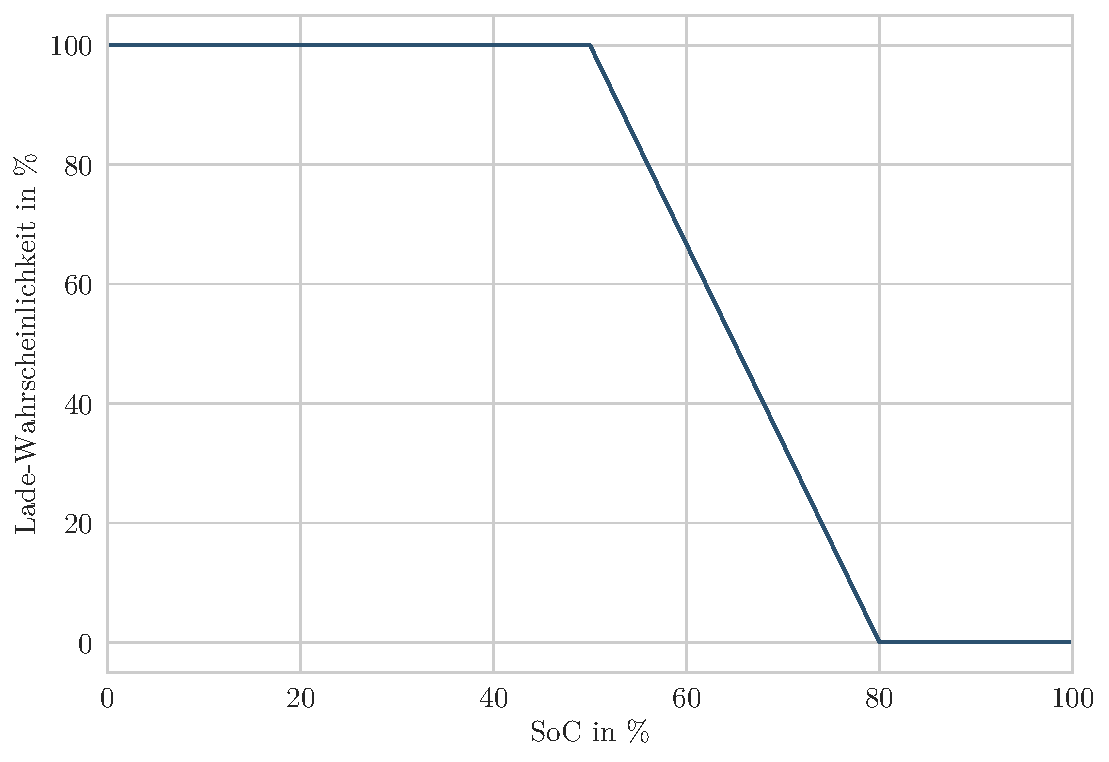
\includegraphics[width=0.9\textwidth]{Bilder/soc_charging_prob}
    \caption{Abhängigkeit der Ladewahrscheinlichkeit vom SoC an öffentlichen Standorten}\label{fig:soc_charging_prob}
\end{figure}

Schnellladeinfrastruktur besitzt aufgrund des zusätzlichen Fahrt- und Zeitaufwandes eine geringere Attraktivität für Fahrzeugnutzer\(^*\)innen.
Deshalb wird eine Schnellladung in dieser Simulation nur dann ausgelöst, wenn es wirklich nötig ist.
Sinkt der \gls{SOC} eines \gls{EPKW} unter \SI{20}{\percent}, wird eine Schnellladestation angefahren und der \gls{EPKW} für \SI{15}{\Minuten} geladen.
Im Unterschied zu \glspl{BEV} können \glspl{PHEV} auch mit einem \gls{SOC} von \SI{0}{\percent} ihre Fahrt mit Hilfe des Verbrennungsmotors fortsetzen.
Aus diesem Grund wird bei \glspl{PHEV} kein Schnellladevorgang ausgelöst.\medskip

Derzeit können mit \glsi{SIMBEV} nur Fahrtprofile mit einer Länge von einer Woche simuliert werden.
Da hierdurch ein Initialproblem eines vollständig geladenen Fahrzeugbestandes am ersten Tag der Simulation dominant hervortritt, wird zu Beginn der Simulation \SI{15}{\percent} der \glspl{EPKW} ein zufälliger \gls{SOC} zwischen \SIrange[range-phrase=~bis~]{30}{100}{\percent} zugeordnet.
Um abschließend ein Fahrtprofil für ein ganzes Jahr zu erhalten, werden die Fahrtprofile solange mit sich selbst verlängert und logisch verknüpft, bis die gewünschte Länge erreicht wird.


\subsubsection{Regionalisierung des Fahrzeugbestandes}

Um die Anzahl an \glspl{EPKW} je \gls{MS}-Netzgebiet zu bestimmen, muss der Gesamtbestand an \glspl{EPKW} je Szenario (s. \autoref{tab:SzenarienRampUp} und \autoref{tab:CarSplit}) regionalisiert werden.
Die Regionalisierung der \glspl{EPKW} findet vorerst auf Ebene der Landkreise statt.
Als Grundlage hierfür dient der aktuelle \textit{PKW-Bestand nach Zulassungsbezirken} \cite[][Stand: \DTMdate{2020-01-01}]{KBAPLZ2020}.
Es wird davon ausgegangen, dass es zu keiner Verschiebung des Bestandanteils zwischen den Zulassungsbezirken kommt.
Dies bedeutet, dass die Gesamtanzahl der \glspl{EPKW} je Fahrzeugklasse und Szenario entsprechend des heutigen Bestandes anteilig verteilt wird.
Die Aufteilung der \glspl{EPKW} in Klassen erfolgt anhand der Einteilung des \gls{PKW}-Bestandes in Hubraum-Klassen, welche ebenfalls dem \textit{PKW-Bestand nach Zulassungsbezirken} entnommen werden können.\medskip

Die geographische Einteilung der Landfläche in \glspl{REGIOSTAR} erfolgt auf Gemeindeebene, weshalb eine weitere Regionalisierung der \glspl{EPKW} innerhalb eines Landkreises auf die jeweiligen Gemeinden notwendig ist.
Da auf Gemeindeebene keine Daten zum \gls{PKW}-Bestand vorliegen, erfolgt die Regionalisierung anhand der Bevölkerungszahl der Gemeinden.
Die Grundlage hierfür bildet der Datensatz \textit{Gemeindegrenzen 2017 mit Einwohnerzahl} \cite[][Stand: \DTMdate{2017-12-31}]{EDG2020}.
Die Verteilung der Anzahl der \glspl{EPKW} erfolgt proportional zur Bevölkerungszahl in der jeweiligen Gemeinde.
Jedes \gls{MS}-Netzgebiet streckt sich dabei in der Regel über mehrere Gemeinden, wobei einzelne Gemeinden auch nur anteilig innerhalb eines Netzgebietes liegen können.\medskip

Um abschließend die Fahrtprofile erzeugen zu können, muss jeder Gemeinde eine \gls{REGIOSTAR} Nummer zugeordnet werden.
Die entsprechende Zuordnung für das Jahr \num{2018} kann dem Datensatz \textit{Referenzdateien zur regionalstatistischen Raumtypologie} \cite[][Stand: \DTMdate{2018-01-01}]{BMVIa2020} entnommen werden.


\subsection{Räumliche Verteilung der Ladevorgänge}\label{chap:theo_distribution}

Die räumliche Verteilung der Ladevorgänge innerhalb eines geographischen Gebietes kann starken Einfluss auf die Auswirkungen der Netzintegration von \glspl{EPKW} haben.
So können beispielsweise regionale Konzentrationen des Ladebedarfs einzelne Leitungen stark beanspruchen und den Netzausbaubedarf erhöhen.
Grundlage für die Ermittlung von möglichen Standorten mitsamt einer Gewichtung bietet eine geoinformatische Auswertung der untersuchten geographischen Gebiete.
Das hierfür verwendete Software Tool wird unabhängig von der vorliegenden Arbeit am \textit{Reiner Lemoine Institut} entwickelt und ist noch nicht veröffentlicht.
Erweiternd zu der Identifizierung der möglichen Ladeinfrastruktur wurde innerhalb dieser Arbeit eine Methodik für die Zuteilung der Ladevorgänge auf die Ladeinfrastruktur entwickelt.
Die Methodik des verwendeten Software Tools und der Zuteilung der Ladevorgänge auf die Ladeinfrastruktur sollen in diesem Kapitel vorgestellt werden soll.\medskip

Innerhalb dieser Arbeit erfolgt die Verteilung der Ladevorgänge immer innerhalb des untersuchten geographischen Gebietes.
In der Realität wird es vorkommen, dass \glspl{EPKW} außerhalb ihres während der Regionalisierung zugewiesenen geographischen Gebietes geladen werden.
Dies betrifft vor allem den Pendel- und Urlaubsverkehr.
Ein Laden in anderen geographischen Gebieten oder das Laden von \glspl{EPKW} aus anderen Gebieten im untersuchten Gebiet kann nicht abgebildet werden.
Es ist anzunehmen, dass sich die hierdurch entstehende Verschiebung des Ladebedarfs zwischen den einzelnen Gebieten ungefähr ausgleichen und keinen großen Einfluss auf die Ergebnisse dieser Untersuchung hat.
In einzelnen Fällen ist ess vorstellbar, dass  auch größere Verschiebungen entstehen, wenn beispielsweise innerhalb eines geographischen Gebietes ein großer Ladepark gebaut wird oder ein großes Unternehmen ansässig ist, welches als Anlaufpunkt für eine Vielzahl von \glspl{EPKW} aus anderen Gebieten dient. 
Ein solcher Fall kann somit nicht innerhalb dieser Arbeit abgebildet werden.


\subsubsection{Private Ladeinfrastruktur}

Die private Ladeinfrastruktur beinhaltet alle Ladevorgänge, die am Eigenheim, in Wohnanlagen oder auf dem Firmenparkplatz stattfinden.
Eine genaue Beschreibung der \UCs findet sich in \autoref{chap:Szenariorahmen}.
Um mögliche Standorte für die Ladeinfrastruktur am Eigenheim oder in Wohnanlagen identifizieren zu können, wird die Anzahl an Wohneinheiten auf einem \SI{100 x 100}{\m} Raster aus dem \textit{Zensus 2011} \cite{StatistischesBundesamt2011} verwendet.
So wird jedem Raster mit mehr als einer Wohneinheit und einer Einwohnerzahl größer Null ein möglicher Anschlusspunkt für Ladeinfrastruktur zugeordnet und anhand der Gesamtanzahl von Wohneinheiten im Raster gewichtet. \medskip

Für private Ladeinfrastruktur auf Firmenparkplätzen werden die Klassifizierungen der Landflächen nach Nutzungsart der \glsi{OSM} \cite{OpenStreetMapFoundation} verwendet.
Hierbei wird jeder Landfläche mit der Nutzungsart \textit{commercial}, \textit{retail} oder \textit{industrial} ein möglicher Anschlusspunkt für Ladeinfrastruktur zugeordnet.
Die Gewichtung erfolgt anhand der Fläche des Gebietes multipliziert mit einem Flächennutzungsfaktor.
Der Flächennutzungsfaktor liegt für \textit{commercial} bei \num{3}, für \textit{retail} bei \num{2} und für \textit{industrial} bei \num{1}.


\subsubsection{Öffentliche Ladeinfrastruktur}

Die öffentliche Ladeinfrastruktur beinhaltet solche, die nicht der privaten Ladeinfrastruktur zugeordnet werden kann.
Grundsätzlich lässt sich hierbei zwischen Normal- und Schnellladeinfrastruktur unterscheiden.
Für die Normalladeinfrastruktur wird allen \glspl{POI} aus der \glsi{OSM} \cite{OpenStreetMapFoundation} in dem untersuchten Gebiet jeweils ein möglicher Anschlusspunkt für Ladeinfrastruktur zugeordnet.
Die Gewichtung der Anschlusspunkte erfolgt hierbei anhand der Gesamtanzahl an \glspl{POI} in der Nähe des Anschlusspunktes.\medskip

Für Schnellladeinfrastruktur wird jeder Tankstelle aus der \glsi{OSM} \cite{OpenStreetMapFoundation} im untersuchten Gebiet jeweils ein Anschlusspunkt zugeordnet.
Liegt innerhalb des Gebietes keine Tankstelle, so wird ein zufälliger Anschlusspunkt der öffentlichen Ladeinfrastruktur verwendet.
Eine Gewichtung findet in diesem Fall nicht statt.


\subsubsection{Zuteilung der Ladevorgänge auf die Ladeinfrastruktur}

Die klassifizierten Landflächen nach Nutzungsart der \glsi{OSM} entsprechen häufig sehr großen Landflächen, die in der Regel nicht nur einem Unternehmen zugewiesen werden können.
Da hierdurch unter Umständen nur wenige Anschlusspunkte generiert werden, werden ergänzend \SI{50}{\percent} der möglichen öffentlichen Normalladeinfrastruktur für Ladeinfrastruktur auf Firmenparkplätzen genutzt.
Den zusätzlichen Anschlusspunkten wird eine geringe Gewichtung zugeordnet, da durch diese vor allem kleine Betriebe abgebildet werden sollen.
Die Gewichtung orientiert sich dabei an der ermittelten Gewichtung der öffentlichen Ladeinfrastruktur.
Bei der privaten Ladeinfrastruktur am Eigenheim oder in Wohnanlagen liegen innerhalb eines Rasters in der Regel mehrere Wohneinheiten, weshalb davon auszugehen ist, dass je identifiziertem Anschlusspunkt mehrere unabhängige Ladepunkte bzw. -parks betrieben werden können.
Auch bei der öffentlichen Normalladeinfrastruktur können unter Umständen mehrere unabhängige Ladepunkte bzw. -parks betrieben werden.
Deshalb werden in diesen drei Fällen die möglichen Anschlusspunkte mehrfach vergeben.
Dabei wird für die Ladeinfrastruktur am Eigenheim oder in Wohnanlagen ein Belegungsfaktor von \num{7}, auf Firmenparkplätzen von \num{5} und für die öffentlichen Normalladeinfrastruktur von \num{2} verwendet.\medskip

Jedem Anschlusspunkt wird vor der Zuteilung der Ladevorgänge eine maximale Anzahl an möglichen Ladepunkten zugeordnet.
Diese entspricht dem Verhältnis von \glspl{EPKW} im \gls{MS}-Netzgebiet und der Anzahl möglicher zuvor ermittelter Anschlusspunkte je \UC multipliziert mit einem Faktor von \num{5}.
Nachdem einem Anschlusspunkt ein Ladepunkt zugeordnet wird, wird die Gewichtung des Anschlusspunktes linear abgesenkt, sodass die Gewichtung des Anschlusspunktes auf Null fällt, sobald die maximale Anzahl an möglichen Ladepunkten erreicht wurde.\medskip

Die Zuteilung der Ladevorgänge auf die Ladeinfrastruktur erfolgt mit Hilfe des Gewichtungsfaktors der Anschlusspunkte.
Dabei erfolgt eine zufällige und gewichtete Auswahl eines Anschlusspunktes je Ladevorgang.
Im Falle der privaten Ladeinfrastruktur wird für jeden \gls{EPKW} ein eigener Ladepunkt eingerichtet.
Diesem Ladepunkt werden alle Ladevorgänge des jeweiligen \glspl{EPKW} und \UC zugeordnet.\medskip

Für die öffentliche Ladeinfrastruktur erfolgt die Zuweisung dezidiert pro Ladevorgang.
So wird je Ladevorgang untersucht, ob bereits ein passender Ladepunkt zur Verfügung steht.
Hierbei wird beachtet, ob in dem entsprechenden Zeitraum der Ladepunkt durch einen anderen \gls{EPKW} besetzt ist und ob dieser die entsprechende Ladeleistung zur Verfügung stellen kann.
Sollte kein passender Ladepunkt zur Verfügung stehen, wird analog zum Vorgehen bei der privaten Ladeinfrastruktur ein Ladepunkt zufällig und gewichtet ausgewählt und eingerichtet.\medskip

Da die \gls{MS}-Netzgebiete nicht immer die Gesamtfläche einer Gemeinde abdecken, muss abschließend geprüft werden, ob die generierten Anschlusspunkte innerhalb des Netzgebietes liegen.
Liegt ein Anschlusspunkt innerhalb eines \gls{MS}-Netzgebietes, so wird er diesem zugeordnet.
Wenn nicht, dann fallen die zugeordneten Ladevorgänge innerhalb eines angrenzenden \gls{MS}-Netzgebietes an und sind somit nicht Teil der abschließenden Auswertungen.


\subsubsection{Netzintegration der Ladeinfrastruktur}

Die Netzintegration der Ladeinfrastruktur erfolgt automatisiert mit Hilfe der \textit{integrate\_component} Funktionalität \glsipl{EDISGO}.
Der Anschluss erfolgt hierbei bis zu einer Anschlussleistung von \SI{0.3}{\mva} in der \gls{NS}-Ebene und bei höheren Anschlussleistungen direkt in der \gls{MS}-Ebene.
Bei einem Anschluss in der \gls{NS}-Ebene erfolgt der Anschluss immer innerhalb des \gls{NS}-Netzes, dessen \gls{MS}-\gls{NS}-\gls{USW} (kurz: \gls{ONS}) am nächsten an dem anzuschließenden Anschlusspunkt liegt.
Ab einer Leistung von \SI{0.1}{\mva} erfolgt der Anschluss über eine Kabelverbindung direkt an der \gls{ONS}.
Unter einer Leistung von \SI{0.1}{\mva} hängt die Art des Anschlusses von dem \textit{use case} der Ladestation ab.
Für den \UC \zH wird die Ladestation an der nächstgelegenen Haushaltslast im identifizierten \gls{NS}-Netz angeschlossen.
Im Falle des \UC \Firmeparkplatz erfolgt der Anschluss an dem nächstgelegenen gewerblichen, industriellen oder landwirtschaftlichen Verbraucher.
Demgegenüber erfolgt im Falle von öffentlicher Ladeinfrastruktur der Netzanschluss der Ladestation an dem nächstgelegen Verbraucher, der keine Haushaltslast darstellt.\medskip

Erfolgt der Anschluss in der \gls{MS}-Ebene, wird die Ladestation über ein Kabel an dem nächstgelegenen Netzknoten oder Kabel angeschlossen.
Hierbei wird ausgeschlossen, dass eine Ladestation an eine andere Ladestation angeschlossen wird.
Wird ein Kabel ausgewählt, wird die Leitung an der nächstgelegenen Stelle zur Ladestation aufgetrennt und eine neue Kabelmuffe hinzugefügt, an welcher die Ladestation angeschlossen wird.
Liegt die Anschlussleistung der Ladestation über \SI{4.5}{\mva}, erfolgt der Anschluss der Ladestation über eine Kabelverbindung direkt an dem \gls{HS}-\gls{MS}-\gls{USW}.\medskip

Es wird angenommen, dass die Anschlussleistung einer Ladestation bis zu einer Leistung von \SI{0.3}{\mva} immer der kumulierten Leistung aller Ladepunkte der Ladestation entspricht.
Ab einem Anschluss in der \gls{MS}-Ebene wird davon ausgegangen, dass immer eine Optimierung der Spitzenlast bei der \UCs \zH und \Firmeparkplatz stattfindet (s. \autoref{chap:theo_strategies}).
Aus diesem Grund wird ab einem Anschluss in der \gls{MS}-Ebene eine Abhängigkeit der Anschlussleistung von der kumulierten Leistung vorgenommen.
Hierbei wird ein linearer Zusammenhang des Anschlussleistungsfaktors von der kumulierten Leistung der Ladepunkte einer Ladestation nach \autoref{fig:connection_rating} angenommen.
Die Anschlussleistung einer Ladestation ergibt sich anschließend aus dem Produkt des Anschlussleistungsfaktors mit der kumulierten Leistung der Ladepunkte der Ladestation.

\begin{figure}[H]
    \centering
    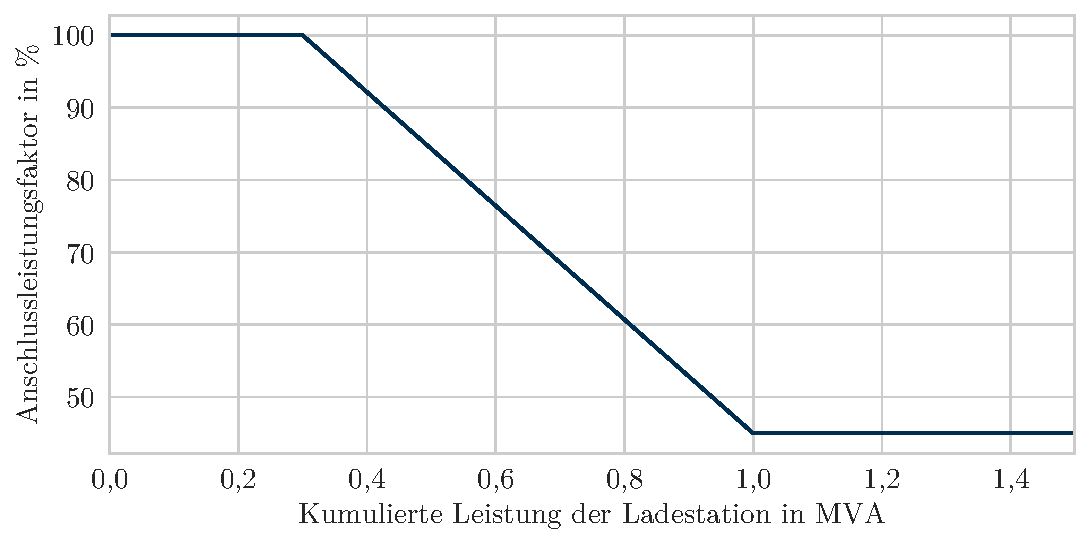
\includegraphics[width=\textwidth]{Bilder/connection_rating_factor}
    \caption{Abhängigkeit des Anschlussleistungsfaktors von der kumulierten Leistung aller Ladepunkte einer Ladestation}\label{fig:connection_rating}
\end{figure}


\subsection{Ladestrategien}\label{chap:theo_strategies}

Innerhalb dieser Arbeit werden zwei präventive Ladestrategien und eine aktive Ladestrategie untersucht.
Auf diese Weise soll analysiert werden, inwieweit eine aktive Ladestrategie gegenüber präventiven Ladestrategien Vorteile aufweist.
Da für aktive Ladestrategien der Aufwand im Betrieb höher ist und zusätzliche Technik benötigt wird, liegen die Kosten für solche Ladestrategien deutlich höher.\medskip

Das Ziel der Ladestrategien ist es, ein möglichst netzfreundliches Verhalten der Ladevorgänge zu erzeugen, ohne den Komfort für Endverbraucher$^*$innen einzuschränken.
Deshalb gilt als Randbedingung aller Ladestrategien, dass der Ladebedarf jedes Ladevorgangs zu \SI{100}{\percent} gedeckt werden muss.
Dies bedeutet, dass Ladevorgänge nur dann flexibilisiert werden können, wenn innerhalb der Standzeit eine Vollladung des \gls{EPKW} möglich ist.
Weiterhin können nur private Ladevorgänge flexibilisiert werden, da bei öffentlichen Ladevorgängen die Erfüllung der Dienstleistung im Vordergrund steht.
Um die drei Ladestrategien bewerten zu können, wird zusätzlich eine Referenz-Ladestrategie untersucht.


\subsubsection{Referenz-Laden}

Bei der Referenz-Ladestrategie wird für Ladevorgänge in der \gls{NS}-Ebene ein vollkommen ungesteuertes Laden der \glspl{EPKW} angenommen.
Da bei großen privaten Ladeparks ein ungesteuertes Laden als unrealistisch einzuschätzen ist, wird davon ausgegangen, dass ab einem Anschluss in der \gls{MS}-Ebene der Betreiber eine Reduktion der Spitzenlast anstrebt.
In diesen Fällen kommt auch bei der Referenz-Ladestrategie das reduzierte Laden zum Einsatz, welches anschließend erläutert wird.


\subsubsection{Ladegruppen}

Das Ziel der Ladegruppen ist es, die Netzbelastung präventiv durch die Senkung der Gleichzeitigkeit der Ladevorgänge zu reduzieren.
Hierfür werden die einzelnen Ladepunkte in zwei Gruppen eingeteilt.
Beiden Gruppen werden alternierend 15-minütige Ladezeitfenster zugewiesen, in denen bei voller Ladeleistung der Ladebedarf gedeckt wird.
Reichen die zugewiesenen Ladezeitfenster nicht aus, um den Ladebedarf des Ladevorgangs zu decken, werden zusätzlich die Ladezeitfenster der anderen Gruppe verwendet, bis der Ladebedarf gedeckt werden kann.
Die Ladezeitfenster der eigenen Gruppe werden dabei priorisiert behandelt.
Es wird darauf geachtet, dass die Zuweisung der Gruppen nicht nur innerhalb eines \gls{MS}-Netzgebietes möglichst leistungshomogen erfolgt, sondern detailliert bis in die einzelnen Stränge der \gls{NS}-Ebene.
Innerhalb eines \gls{NS}-Stranges wird weiterhin darauf geachtet, dass auch die einzelnen Leistungsklassen der Ladeinfrastruktur gleichmäßig auf die Gruppen verteilt werden.
Erfolgt der Anschluss einer Ladestation auf der \gls{MS}-Ebene, wird diese Ladestation wie ein eigener \gls{NS}-Strang behandelt und die einzelnen Ladepunkte dementsprechend in die Gruppen eingeteilt.
In \autoref{fig:group_vis} wird beispielhafte die Einteilung von Ladepunkten auf die zwei Gruppen innerhalb eines \gls{NS}-Stranges dargestellt. \cite{Schachler2021}

\begin{figure}[H]
    \centering
    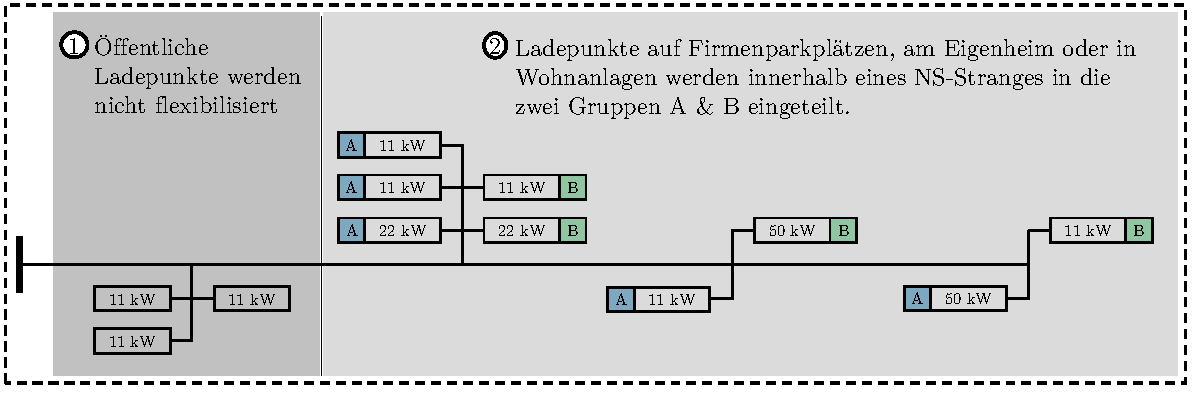
\includegraphics[width=\textwidth]{Bilder/grouped_charging_vis_cropped}
    \caption{Einteilung der Ladepunkte eines NS-Stranges in die Gruppen A und B für das gruppierte Laden}\label{fig:group_vis}
\end{figure}


\subsubsection{Reduziertes Laden}

Beim reduzierten Laden soll präventiv durch die Reduzierung der Ladeleistung der einzelnen Ladevorgänge eine Senkung der Netzbelastung erreicht werden.
Hierbei wird durch eine Absenkung der Ladeleistung möglichst die gesamte Standzeit des \gls{EPKW} für den Ladevorgang genutzt.
Die Flexibilität dieser Ladestrategie wird durch eine Mindestladeleistung von \SI{10}{\percent} der Nennleistung des angefahrenen Ladepunktes technisch begrenzt.
Hierdurch soll ein Kompromiss zwischen einer möglichst großen Reduktion der Ladeleistung und den technischen Anforderungen der Ladeinfrastruktur gefunden werden.
Im Gegensatz zur Referenz-Ladestrategie werden unabhängig von der Netzebene beim reduzierten Laden alle privaten Ladevorgänge flexibilisiert. \cite{Schachler2021}


\subsubsection{Residuallast-Laden}

Bei dem Residuallast-Laden handelt es sich um eine aktive Ladestrategie, welche an das gesteuerte Laden der Agora Studie \textit{Verteilnetzausbau für die Energiewende} \cite{Agora2019} angelehnt ist.
Der Ladevorgang eines \gls{EPKW} findet hierbei immer innerhalb der Zeitschritte der Standzeit statt, welche die geringste Residuallast innerhalb des \gls{MS}-Netzgebietes aufweisen, wodurch eine Glättung der Residuallast erreicht werden soll.
Die Zuweisung findet auf Viertelstundenbasis und die Ladevorgänge immer bei voller Ladeleistung statt.
Das Ziel der Optimierung kann so formuliert werden, dass nach \autoref{eq:residual} eine Minimierung der \glspl{MQA} der Residuallast vom Mittelwert der Residuallast angestrebt wird.

\begin{equation}
	\text{MQA} = \frac{1}{n} \sum_i^n \left( P_{\text{R}_i} - \overline{P}_{\text{R}} \right)^2
	\label{eq:residual}
\end{equation}

\noindent Wobei:

\addvbuffer[12pt 12pt]{
	\begin{tabular}{>{$}r<{$}@{\ :\ }l}
		P_{\text{R}_i}				& Residuallast zum Zeitschritt $i$  \\
		\overline{P}_{\text{R}}		& Mittelwert der Residuallast 		\\
		n							& Anzahl an Zeitschritten			\\
		i							& Index des Zeitschrittes 			\\
	\end{tabular}
}

Durch die Abhängigkeit der Residuallast von den einzelnen Ladevorgängen sind auch die einzelnen Ladevorgänge voneinander abhängig.
Hierdurch entsteht ein komplexes Optimierungsproblem.
Um die Rechenzeit in einem akzeptablen Maß zu halten, wird eine Näherung an eine optimale Lösung angestrebt.
Für jeden Ladevorgang wird ermittelt, wie viel überschüssige Standzeit zur Flexibilisierung der Ladevorgänge zur Verfügung steht.
Die Ladevorgänge werden anschließend in Abhängigkeit dieses Kriteriums in aufsteigender Reihenfolge sortiert und einzeln betrachtet.
So werden für jeden Ladevorgang die Zeitschritte für den Ladevorgang ausgewählt, welche innerhalb der Standzeit die geringste Residuallast aufweisen.
Zusätzlich wird die Residuallast nach jeder Zuweisung entsprechend angepasst und somit die Abhängigkeit der einzelnen Ladevorgänge voneinander gewährleistet.
Auf diese Weise werden Ladevorgänge mit einem geringen Flexibilitätsband vorrangig behandelt und eine möglichst optimale Lösung bei einem geringen Rechenaufwand erreicht.


\subsection{Überführung der Fahrtprofile in Lastzeitreihen}

Die Fahrtprofile der \gls{EPKW} und die Lastzeitreihen der Ladestrategien werden auf \SI{15}{\Minuten} Basis generiert.
In vielen Zeitschritten kann der {--} verbleibende {--} Ladebedarf in weniger als \SI{15}{\Minuten} nachgeladen werden.
Aus diesem Grund wird durch zwei Maßnahmen ein Kompromiss angestrebt.
Einerseits sollen realistische Gleichzeitigkeiten abgebildet werden, welche Auswikungen auf die Netzbelastung haben.
Andererseits soll die Differenz zwischen dem Ladebedarf der Fahrtprofile nach \glsi{SIMBEV} und den Lastzeitreihen der Ladestrategien minimal ausfallen.

\begin{enumerate}
	\item Dem Gesamtladebedarf eines Ladevorgangs wird nur dann der Ladebedarf des letzten Zeitschritts zugeordnet, wenn bei maximaler Ladeleistung mindestens \SI{20}{\percent} des Zeitschritts benötigt werden, um den Ladebedarf zu decken.
	\item Wenn einem Ladevorgang der Ladebedarf des letzten Zeitschritts zugeordnet wird, dann wird in allen für die Ladung auch nur anteilig benötigten Zeitschritten dies in den Lastzeitreihen durch die zugewiesene Ladeleistung des Ladevorgangs in voller Höhe widergespiegelt.
\end{enumerate}

Wenn ein Ladevorgang von diesen Maßnahmen betroffen ist, dann wird der Ladebedarf dieses Ladevorgangs entweder erhöht oder reduziert in den Lastzeitreihen wiedergegeben.
Bei dem reduzierten Laden entsteht diese Problematik bei den flexibilisierbaren Ladevorgängen nicht, da sich die Ladeleistung flexibel nach dem gegebenen Ladebedarf und der zur Verfügung stehenden Standzeit ausrichten kann.
Hierdurch entsteht jedoch eine Differenz in dem Gesamtenergiebedarf der Lastzeitreihen zwischen dem reduzierten Laden und den sonstigen Ladestrategien.
Um dies zu vermeiden werden die zuvor beschriebenen Maßnahmen vor der Erstellung der Lastzeitreihen durchgeführt und der Ladebedarf bereits in den Fahrtprofilen nach \glsi{SIMBEV} angepasst.
Auf diese Weise wird sichergestellt, dass sich der Gesamtenergiebedarf der Lastzeitreihen zwischen den Ladestrategien nicht unterscheidet.
Dies soll kurz an zwei Beispielen veranschaulicht werden:

\begin{enumerate}
	\item Beträgt der Ladebedarf eines Fahrzeuges nach \glsi{SIMBEV} beispielsweise \SI{12}{\kwh} und die fahrzeugseitige Wirkleistung \SI{9.9}{\kw}, dann werden insgesamt rund \SI{73}{\Minuten} für die Ladung benötigt. In diesem Fall wird in den Lastzeitreihen insgesamt fünf Zeitschritten und somit \SI{75}{\Minuten} die Ladeleistung zugeordnet. Aus diesem Grund wird der Ladebedarf des Ladevorgangs in den Fahrtprofilen nach \glsi{SIMBEV} auf \SI{12.375}{\kwh} erhöht.
	\item Wenn hingegen der Ladebedarf bei einer gleichbleibenden Ladeleistung nur \SI{10}{\kwh} beträgt, dann werden nur rund \SI{61}{\Minuten} für die Ladung benötigt. In diesem Fall wird die Ladeleistung in den Lastzeitreihen nur in vier Zeitschritten und somit \SI{60}{\Minuten} abgebildet. Der Ladebedarf des Ladevorgangs in den Fahrtprofilen nach \glsi{SIMBEV} wird entsprechend auf \SI{9.9}{\kwh} reduziert.
\end{enumerate}


\subsection{Netzuntersuchung}\label{chap:edisgo_theo}

Das Open Source Tool \glsi{EDISGO} stellt eine Toolbox zur Verfügung, um Verteilnetze auf Netzprobleme zu untersuchen.
Dabei bilden synthetische Netztopologien, die mit Hilfe des Open Source Tools \glsi{DINGO} erzeugt wurden, die Grundlage für die Berechnungen.
\glsi{EDISGO} kann über \textit{GitHub} \cite{edisgoGit2019} abgerufen werden und ist auf \textit{Read the Docs} \cite{edisgoDocs2017} dokumentiert.\medskip

Mit Hilfe \glsipl{EDISGO} werden vorerst durch eine Lastflussanalyse Netzprobleme in den Referenznetzgebieten ermittelt.
Anschließend wird der last- und erzeugerseitigen Abregelungsbedarfs ermittelt, welcher nötig ist, um die Netzprobleme aufzulösen.
Anhand dieses Wertes sollen Aussagen darüber gemacht werden, inwieweit die Ladestrategien dazu in der Lage sind, kritische Netzbelastungen zu vermeiden beziehungsweise zu reduzieren.
Gegenüber einer Ermittlung der Netzausbaukosten bringt diese Methodik den Vorteil mit sich, dass Aussagen darüber getroffen werden können, ob die Netzprobleme aufgrund von einer zu starken Last oder Einspeisung entstehen.


\subsubsection{Ermittlung von Netzproblemen}\label{chap:grid_issues}

Die Überprüfung der Referenznetzgebiete auf Netzprobleme besteht aus zwei Schritten.
Vorerst wird eine nichtlineare Lastflussanalyse durchgeführt, um anschließend die Einhaltung der Spannungsanforderungen und technischen Richtlinien bezüglich der Betriebsmittelbelastungen zu überprüfen.
Die Durchführung der Lastflussanalyse erfolgt mit Hilfe \glsipl{EDISGO}, welches die Funktionalitäten des Open Source Tools \textit{PyPSA} \cite{Brown2020} nutzt.
In diesem Kapitel soll auf den Umfang der Lastflussanalyse und die Spannungsanforderungen sowie die technischen Richtlinien bezüglich der Gerätebelastungen eingegangen werden.
Eine genau Beschreibung der Lastflussanalyse des Open Source Tools \textit{PyPSA} kann auf \textit{Read the Docs} \cite{Brown2020a} abgerufen werden.\medskip

Die Lastflussanalyse der Netze berücksichtigt sowohl \gls{MS}- und \gls{NS}-Leitungen als auch die \gls{MS}-\gls{NS}-Umspannebene.
Gegenüber einer Aggregation der Erzeugung und des Bedarfs der einzelnen \gls{NS}-Netze an der jeweiligen \gls{ONS} bietet diese tiefgehende Betrachtung die Möglichkeit, die Auswirkungen der teilweise hohen Ladeleistungen der Ladeinfrastruktur genauer zu analysieren und den Einfluss verschiedener Ladestrategien umfassender bestimmen zu können.\medskip

Unter dem Bilanzknoten wird ein Netzknoten verstanden, an welchem der Wirk- und Blindleistungsfluss frei eingestellt werden kann, womit über einen iterativen Prozess bei der Lastflussanalyse die Konvergenz des Systems erreicht werden soll.
Da die Spannung der Sekundärseite des \gls{HS}-\gls{MS}-\glspl{USW} auch in der Realität eingestellt werden kann, eignet sich dieser Punkt besonders gut und wird entsprechend als Bilanzknoten verwendet.
Aus diesem Grund können am \gls{HS}-\gls{MS}-\gls{USW} keine Spannungsprobleme auftreten.
Jedoch entspricht die bei der Lastflussanalyse berechnete Scheinleistung des Bilanzknotens der Leistung, die über das \gls{HS}-\gls{MS}-\gls{USW} geleitet wird.
Anhand dieses Wertes können erweiternd Aussagen über etwaige Überlastungen des \gls{HS}-\gls{MS}-\glspl{USW} getroffen werden.
In \autoref{fig:scope} ist eine Übersicht über den Umfang der Lastflussanalyse dargestellt. \cite{Schachler}

\begin{figure}[H]
    \centering
    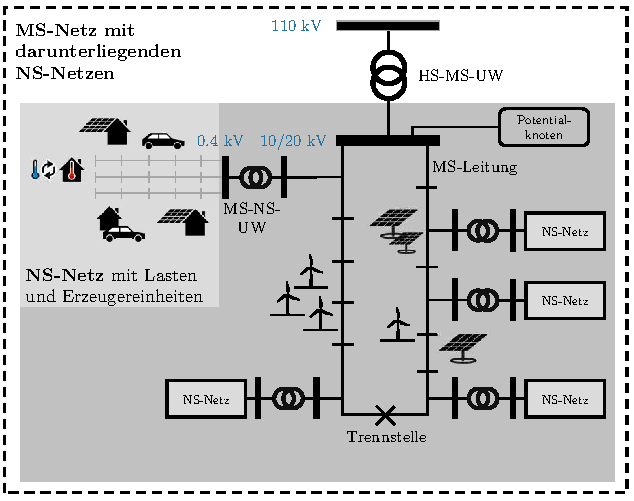
\includegraphics[width=\textwidth]{Bilder/scope_power_flow_kh_cropped}
    \caption[Umfang der Lastflussanalyse mit eDisGo]{Umfang der Lastflussanalyse mit eDisGo \cite{Schachler}}\label{fig:scope}
\end{figure}

Mit Hilfe der durch die Lastflussanalyse ermittelten Belastungen und Spannungsabweichungen an den Betriebsmitteln können abschließend Überlastungen und Spannungsprobleme festgestellt werden.
Im Rahmen dieser Arbeit gilt als Planungsgrundsatz, dass der auf Scheinleistung bezogene zulässige Belastungsfaktor aller Betriebsmittel \SI{100}{\percent} beträgt.
Die zulässigen Spannungsabweichungen liegen für Endkunden in der \gls{NS}-Ebene bei \SI{\pm 10}{\percent}.
Dieses Spannungsband wird nach \autoref{tab:Spannungsband} auf die \gls{MS}, \gls{MS}-\gls{NS}- und \gls{NS}-Ebene aufgeteilt.
Im Lastfall spiegelt das in der \gls{NS}-Ebene größere zulässige Spannungsband wider, dass in dieser Ebene die Mehrzahl der Verbraucher angeschlossen ist.
Demgegenüber wird im Rückspeisefall ein größeres Spannungsband für die \gls{MS}-Ebene reserviert.
Die Aufteilung des zulässigen Spannungsbandes nach \autoref{tab:Spannungsband} wird aus \textit{Integrated Techno-Economic Power System Planning of Transmission and Distribution Grids} \cite{Mueller2019a} entnommen und basiert auf der \textit{Verteilnetzstudie für das Land Baden-Württemberg} \cite{Rehtanz2017}

{
\renewcommand{\arraystretch}{1.2}% grßerer Zeilenabstand
\sisetup{range-phrase=~bis~}
\begin{table}[H]
	\begin{center}
		\caption{Zulässige Spannungsabweichungen der Betriebsmittel in der MS- und NS-Ebene}
		\begin{tabu} to 0.5\textwidth {X[1.2] X[1, r] X[1, r]}
			\toprule
			Spannungsebene & Lastfall               & Rückspeisefall             \\ \midrule
			MS             & \SI{-1.5}{\percent}    & \SI[retain-explicit-plus]{+5.0}{\percent}   	 \\
			MS-NS          & \SI{-2.0}{\percent}    & \SI[retain-explicit-plus]{+1.5}{\percent}   	 \\
			NS             & \SI{-6.5}{\percent}    & \SI[retain-explicit-plus]{+3.5}{\percent}   	 \\ \bottomrule
            \multicolumn{3}{l}{Quelle: \cite{Rehtanz2017}}
		\end{tabu}
		\label{tab:Spannungsband}
	\end{center}
	\vspace{-3mm}%Put here to reduce too much white space after your table
\end{table}
}


\subsubsection{Ermittlung des Abregelungsbedarfs für die Auflösung von Netzüberlastungen}

Die Ermittlung des Abregelungsbedarfs für die Auflösung von Spannungsbandverletzungen und Betriebsmittelüberbelastungen erfolgt in einem iterativen Prozess.
Vorerst werden etwaige Netzprobleme und die entsprechenden Zeitschritte, in denen die Netzprobleme auftreten, mit Hilfe der Lastflussanalyse ermittelt.
Anschließend wird die Last bzw. die Einspeisung in \SI{5}{\percent}-Schritten innerhalb der ermittelten Zeitschritte reduziert.
Beides wird so lange wiederholt, bis keine Netzprobleme mehr auftreten.\medskip

Bei der Lösung der Netzprobleme werden vorerst Spannungsprobleme und abschließend Überlastungen behandelt.
Weiterhin werden Probleme in der \gls{NS}-Ebene behandelt, bevor Probleme in der \gls{MS}-\gls{NS}-Umspannebene und abschließend in der \gls{MS}-Ebene gelöst werden.
Durch die Auflösung von Netzproblemen auf tieferen Spannungsebenen können unter Umständen bereits Netzprobleme in darüber liegenden Spannungsebenen gelöst, entspannt oder auch verstärkt werden.
Weiterhin werden Netzprobleme innerhalb der \gls{NS}- bzw. \gls{MS}-Ebene anhand ihrer Entfernung zur übergeordneten Umspannebene priorisiert.
So kann auch hier die Lösung von weiter entfernten Netzproblemen bereits vorgeschaltete Netzprobleme auflösen oder entspannen.
Für jeden Zeitschritt, in dem Überlastungs- oder Spannungsprobleme an einem Netzknoten auftreten, wird geprüft, ob die Netzprobleme durch hohe Nachfrage oder hohe Einspeisung entstehen.
Anhand dieser Information wird entschieden, ob Last oder Einspeisung abgeregelt werden soll.
Die gesamte notwendige Abregelung für das \gls{MS}-Netzgebiet ergibt sich aus der Summierung aller nötigen Abregelungen von Last und Erzeugung.
In \autoref{fig:scope_curtailment} ist das Vorgehen veranschaulicht. \cite{Schachler}

\begin{figure}[H]
    \centering
    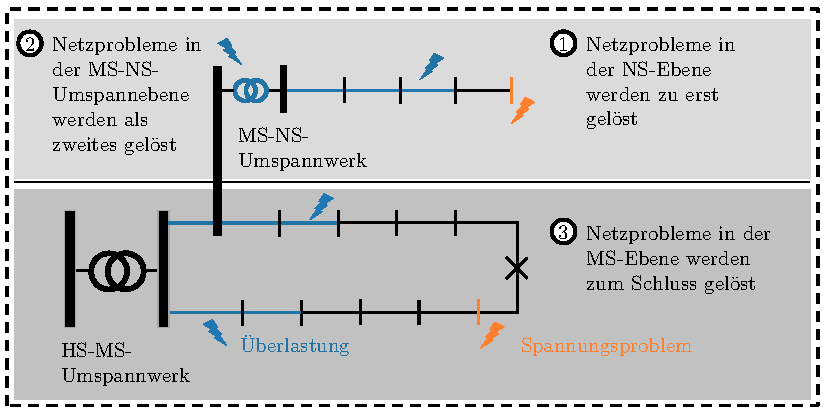
\includegraphics[width=\textwidth]{Bilder/grid_issues_scope_cropped}
    \caption[Umfang der Ermittlung des Abregelungsbedarfs für die Auflösung von Spannungsbandverletzungen und Betriebsmittelüberbelastungen]{Umfang der Ermittlung des Abregelungsbedarfs für die Auflösung von Netzüberlastungen \cite{Schachler}}\label{fig:scope_curtailment}
\end{figure}

Um die Rechenzeit innerhalb eines akzeptablen Maßes zu halten, erfolgt die Ermittlung des Abregelungsbedarfs für zwei Wochen des Jahres.
Hierbei werden die Wochen untersucht, die im \gls{MS}-Netzgebiet die minimale bzw. maximale durchschnittliche Residuallast aufweisen.
Auf diese Weise sollen möglichst extreme Belastungssituationen abgedeckt werden.\medskip

Aufgrund der hohen Anzahl an \glspl{EPKW}, \glspl{WP} und Erneuerbaren Erzeugereinheiten kommt es in einigen Fällen dazu, dass die Lastflussanalyse nicht konvergiert.
Aus diesem Grund werden zuerst die \gls{NS}-Netze eines \gls{MS}-Netzgebiets einzeln betrachtet und bei Bedarf abgeregelt, um dort extreme Belastungssituationen abzufangen, die eine Konvergenz des Gesamtsystems verhindern können.

\clearpage
